% CC⇌WM Interconversion — paper skeleton (ICLR/NeurIPS or TMLR style)
\documentclass[10pt]{article}
\usepackage[a4paper,margin=1in]{geometry}
\usepackage{amsmath,amssymb,graphicx,booktabs,natbib,hyperref}
\title{Claim-Chain $\rightleftharpoons$ World-Model Interconversion:\\
The Common Key Technology Bridging Simulation and Symbolic Cognition for Vibe Research}
\author{Anonymous}
\begin{document}
\maketitle

\begin{abstract}
Vibe research---autonomous modeling, control design, and platform design---requires
\emph{both} a simulation-capable world model (physical perception) and a claim chain
(symbolic cognition / writing). We study \textbf{CC$\rightleftharpoons$WM interconversion}
as the \emph{common key technology} that bidirectionally bridges them: a faithful,
round-trippable mapping between a JEPA world model and a structured claim chain.
We formalize the interconversion, give SOTA conversion algorithms
(causal WM$\to$CC extraction via probing$\to$selectivity$\to$DAS interchange intervention;
effective+preserving CC$\to$WM compilation via semantic loss + KG-as-architectural-prior
+ Rho-routed hard/soft constraints + a LoRA/EWC/bisimulation fidelity stack), and validate
three claims on LeWorldModel: (C1) the conversion is well-defined and faithful;
(C2) round-trip fidelity is high (information $\Delta I$ and behavioral Wasserstein stay
bounded); (C3) the \emph{same} CC$\rightleftharpoons$WM substrate serves both a
simulation-side task and a writing-side task---establishing it as the shared backbone
for future vibe-research systems.
\end{abstract}

\section{Introduction}
% vibe research needs sim + writing; no common substrate; CC⇌WM is it.
% contributions: C1 formalization+mechanism, C2 fidelity, C3 common substrate.

\section{Related Work}
% ENPIRE (memoryless auto-research), FLUXturbo/Sym2Real (one-directional),
% Two-Paths-NS-JEPA (training-time fusion), Dreamer/JEPA probing (Garrido/LeWM),
% DAS (Geiger), Semantic Loss/LTN/Scallop, LoRA/EWC/MIMKD, bisimulation.

\section{CC$\rightleftharpoons$WM Interconversion}
\subsection{Formal definition}
% WM = (encoder, predictor, latent z); CC = (atoms, typed edges, Rho).
% Interconversion = pair of maps extract: WM→CC, compile: CC×WM→WM'.
\subsection{WM$\to$CC extraction (causal)}
% probe R² → selectivity (control task) → completeness → DAS/IIA interchange intervention
% → SINDy-SHRED latent dynamics → surprise/OOD boundary; 7 faithfulness metrics.
\subsection{CC$\to$WM compilation (effective + preserving)}
% semantic loss / LTN / Scallop; KG-as-architectural-prior (typed edges → predictor wiring);
% Rho.confidence routes hard (equivariant/hPINN) vs soft (GradNorm); fidelity stack
% (freeze encoder + LoRA + EWC + MIMKD-MI distillation + latent bisimulation).
\subsection{Round-trip fidelity}
% 3-layer (info cosine-R² / behavioral pred-MSE / logical) + MI-gap ΔI + latent Wasserstein;
% DPI upper bound; single-direction held-out guard.

\section{Experimental Setup}
% LeWorldModel on DMC reacher (single WM case, depth over breadth);
% probes, DAS, compile-back, fidelity metrics, seeds.

\section{Results}
\subsection{C1: extraction is faithful and causal}
% Fig: per-quantity R² + DAS IIA vs null (Fig. \ref{fig:das}).
\subsection{C2: round-trip is fidelity-preserving}
% Fig: 3-layer fidelity + ΔI + W1 (Fig. \ref{fig:fidelity}).
\subsection{C3: common substrate}
% same CC⇌WM runs sim-side (modeling) + write-side (hypothesis$\to$evaluation$\to$writing).
\subsection{Compilable vs architecturally-uncompilable}
% Fig: qpos² (compilable, R²↑) vs qvel (uncompilable, unobservable) (Fig. \ref{fig:compile}).

\section{Ablations}
% probe type (linear/MLP/DAS); selectivity; compile λ/epochs; LoRA rank; round-trip depth.

\section{Limitations}
% single WM case (depth over breadth); linear-subspace DAS; SAE/Scallop/bisimulation depth.

\section{Conclusion}
% CC⇌WM as the common substrate unifying simulation and writing for vibe research
% (modeling/control/platform-design outlook).

\begin{figure}[h]\centering
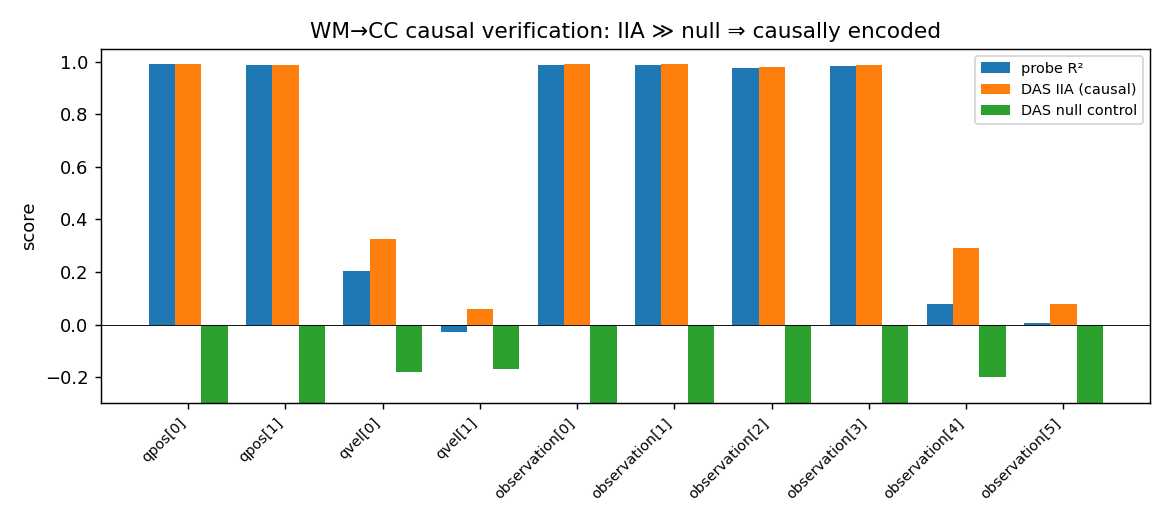
\includegraphics[width=0.9\linewidth]{fig_das.png}
\caption{WM$\to$CC causal verification: per-quantity probe R$^2$ vs DAS interchange-accuracy
IIA vs null-direction control. High IIA $\gg$ null $\Rightarrow$ causally encoded.}
\label{fig:das}\end{figure}

\begin{figure}[h]\centering
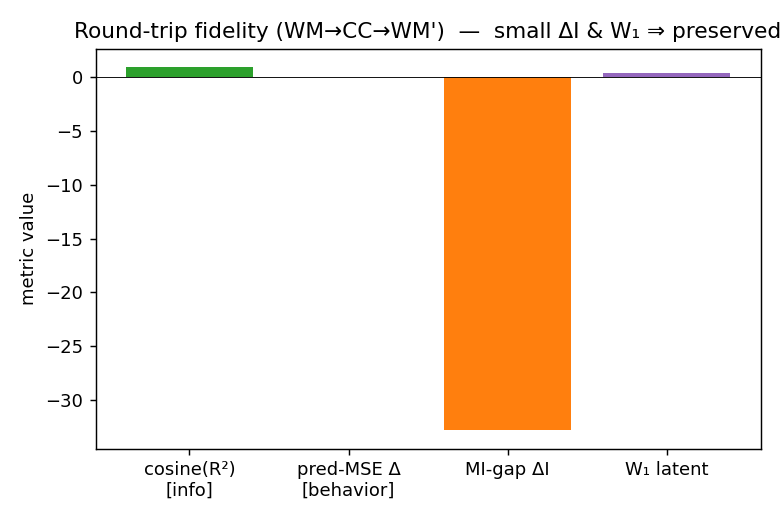
\includegraphics[width=0.9\linewidth]{fig_fidelity.png}
\caption{Round-trip fidelity: info-layer cosine(R$^2$), behavioral pred-MSE, MI-gap $\Delta I$,
latent Wasserstein $W_1$. Small $\Delta I$ and $W_1$ $\Rightarrow$ interconversion preserves
information and behavioral distribution.}
\label{fig:fidelity}\end{figure}

\begin{figure}[h]\centering
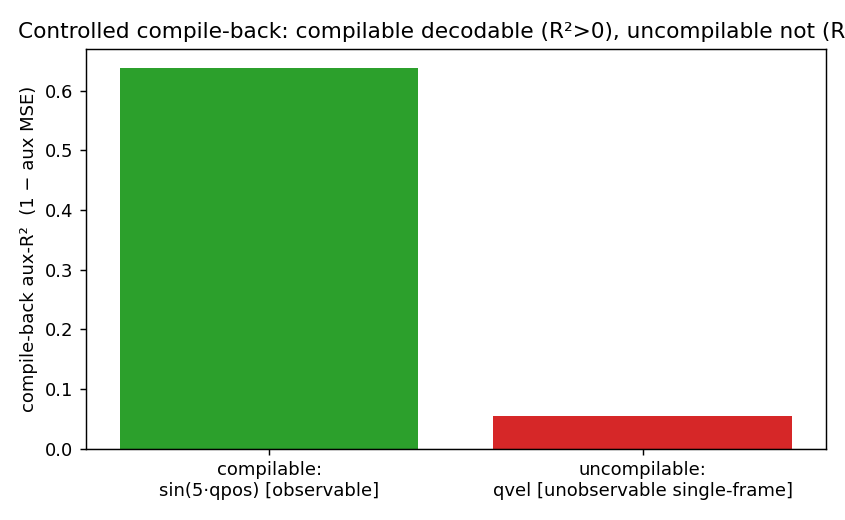
\includegraphics[width=0.9\linewidth]{fig_compile.png}
\caption{Controlled compile-back: compilable target (qpos$^2$, observable) R$^2$ rises after
CC$\to$WM compilation while fidelity is preserved; uncompilable target (qvel, unobservable
single-frame) does not---an architectural limit, not a capacity gap.}
\label{fig:compile}\end{figure}

\bibliographystyle{plainnat}
\bibliography{refs}
\end{document}
